\documentclass{article}

\usepackage{mhchem}
\usepackage{siunitx}
\usepackage{graphicx}
\usepackage{caption}
\usepackage{amsmath}
\usepackage{amsfonts}
\usepackage{physics}
\usepackage{url}

\newcommand{\cc}{$\,\text{cm}^{3}$}
\newcommand{\circa}{\emph{circa }}
\newcommand{\g}{\,g}

\title{Macroscopic AFM -- Plan}
\date{01/12/2020}
\author{Samuel Frost}

\begin{document}

\maketitle

\section*{Preliminary Knowledge}
AFM is commonly used to find imformation about the surface of an object, passing over microscopic mountains and 
trenches. To ensure the tip is able to detect these properly it has to be thinner than the trough that it is scanning
so that it can reach the bottom (or near it in non-contact mode) and thus determine the depth. The average tip 
size is only 20\,nm, and can be made from a range of materials, however silicon based ones are most common. 

\subsection*{Contact Mode}
In contact mode the tip is dragged across the surface of the material, to minimise damage this is done at a distance 
where the force from the surface is repulsive. This still leads to lots of problems, the tip is can become damaged and 
as such the same reading will give different results when taken at a later time; with delicate matierals such
as biological samples, contact mode can permanently damage them. 

\begin{figure}[h]
    \centering
    \captionsetup{justification=centering}
    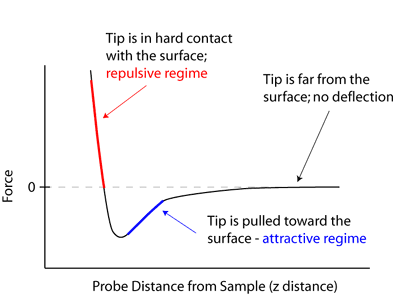
\includegraphics[width=6cm]{AFM.png}
    \caption{Force-distance curve for an AFM tip\cite{curve}}
\end{figure}

\subsection*{Non-contact mode}
To avoid such fates a new method was devised, non-contact mode. The cantilever is oscilated at its resonant 
frequency, when in close proximity to the surface van der Waals forces attract the tip, this decreases its resonant
frequency and from this data a surface can be plotted. 

\section*{Plan}

The aim of this experiment is to show how the principles of an Atomic Force Microscope still apply at the 
macroscopic level. To collect similar data and show how this would be applied at the nanoscale. 

The fundamental frequeny of the steel cantilever can be determined from the following equation:
$$f_m = C_m\left(\frac{EI}{\mu l^4}\right)^{\frac{1}{2}}$$
\begin{itemize}
    \item $m \in \mathbb{N}$
    \item $C_1 = 0.5596, C_2 = 3.5069$
    \item $E = 190 \pm 20$ GPa is the Young's modulus for steel
    \item $\mu = 0.042 \pm 0.005$ kgm is the density of steel
    \item $l = 208 \pm 1$ mm is the length of the cantilever
    \item $I = \frac{bd^3}{12}$ is the moment of inertia of the cantilever
    \item $b = 4.25 \pm 0.01$ mm is shown in the diagram below in Figure: \ref{bd}
    \item $d = 1.50 \pm 0.01$ mm is again shown below in Figure: \ref{bd}
\end{itemize}

$$\frac{C_2}{C_1} = \frac{f_2}{f_1} = 2\pi$$
The ratio between the frequencies is 2$\pi$, this differes from a standing wave where the ratio is 2.

In order for this equation to be valid the force exerted by the surface, or the \emph{stress} exerted on the 
cantilever must be elastic, the metal cannot plastically deform. The stress vs strain graph must not 
go past the yield strength point marked in Figure: \ref{young}. 
\begin{align*}
    \text{Stress,\ } \sigma &= \frac{Force}{Area}\\
    \text{Strain,\ } \epsilon &= \frac{\Delta l}{l_0}
\end{align*}

Where $\Delta l$ is the change in length of the material and $l_0$ is the original length before any stress is 
exerted.

\begin{figure}[h]
    \centering
    \captionsetup{justification=centering}
    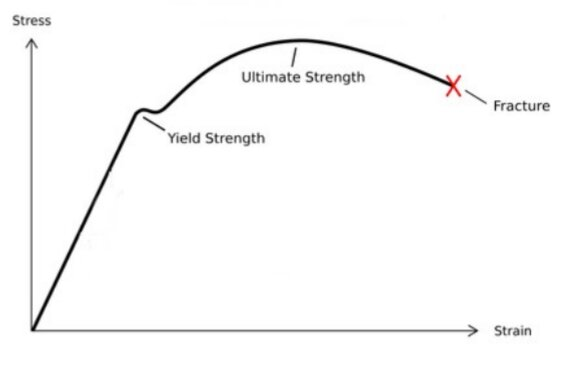
\includegraphics[width=6cm]{young.jpg}
    \caption{Stress vs Strain for a ductile matieral \label{young}}
\end{figure}

\begin{figure}[h]
    \centering
    \captionsetup{justification=centering}
    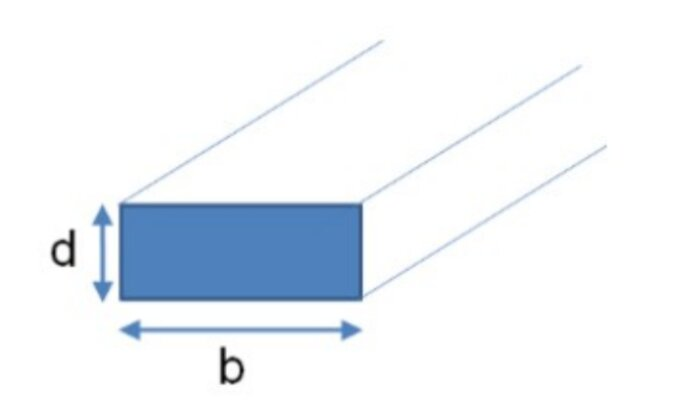
\includegraphics[width=6cm]{bd.jpg}
    \caption{Definition of b and d \label{bd}}
\end{figure}

Note that the values of $b, d$ and $l$ will vary for the actual experiment and so will have to be measured.
Finding the funamnetal frequnecy ($f_1$) of this hypothetical cantilever gives us.
$$f_1 = 30 \pm 2.43\text{\,Hz} $$
$$f_2 = 188.5 \pm 15.27\text{\,Hz}$$
This is quite a wide margin of uncertainty, however it is accurate enough to give us a rough region of where to locate
the fundamnetal frequency, from the beginning of this region fine increments can be used to find the exact measuremeant.

The uncertainty was found through the following formula
\begin{align*}
    \delta f &= \sqrt{\left(\pdv{f}{\mu}\delta\mu\right)^2 + \left(\pdv{f}{E}\delta E\right)^2 + \ldots}\\
    C &= \frac{1}{2}C_1(f_1)^{-\frac{1}{2}} = 5.2 \cdot 10^{-3}\\
    \left(\pdv{f}{\mu}\delta\mu\right) &= -C \frac{Ebd^3}{12\mu^2l^4}\delta\mu = -1.788\\
    \left(\pdv{f}{l}\delta l\right) &= -C \frac{4Ebd^3}{12\mu^2l^5}\delta l = -0.288\\
    \left(\pdv{f}{E}\delta E\right) &= C \frac{bd^3}{12 \mu^2l^4}\delta E = 1.581\\
    \left(\pdv{f}{b}\delta b\right) &= C \frac{Ed^3}{12\mu^2l^4}\delta b = 0.0353\\
    \left(\pdv{f}{d}\delta d\right) &= C \frac{3Ebd^2}{12\mu^2l^4}\delta d = 0.3\\
    \delta f &= 2.43 \text{Hz} 
\end{align*} 

\subsection*{Experiment}
\begin{enumerate}
    \item Measure the dimensions of the cantilever ($b$ and $d$) and note the uncertainty. 
    \item Set up the experiment as seen in Figure: \ref{fig}. Ensure there is no magnet beneath the cantilever tip and vary the signal of the oscilator until 
    a rough region of resonance frequency is found. Start recording data before this region, record the 
    amplitude the laser makes on the wall and the frequency at which this occurs. Record data in finer steps 
    as the amplitude begins to increase quicker. Note the uncertainty of the oscilator and graph paper used to 
    find the amplitude. 
    \begin{figure}[h]
        \centering
        \captionsetup{justification=centering}
        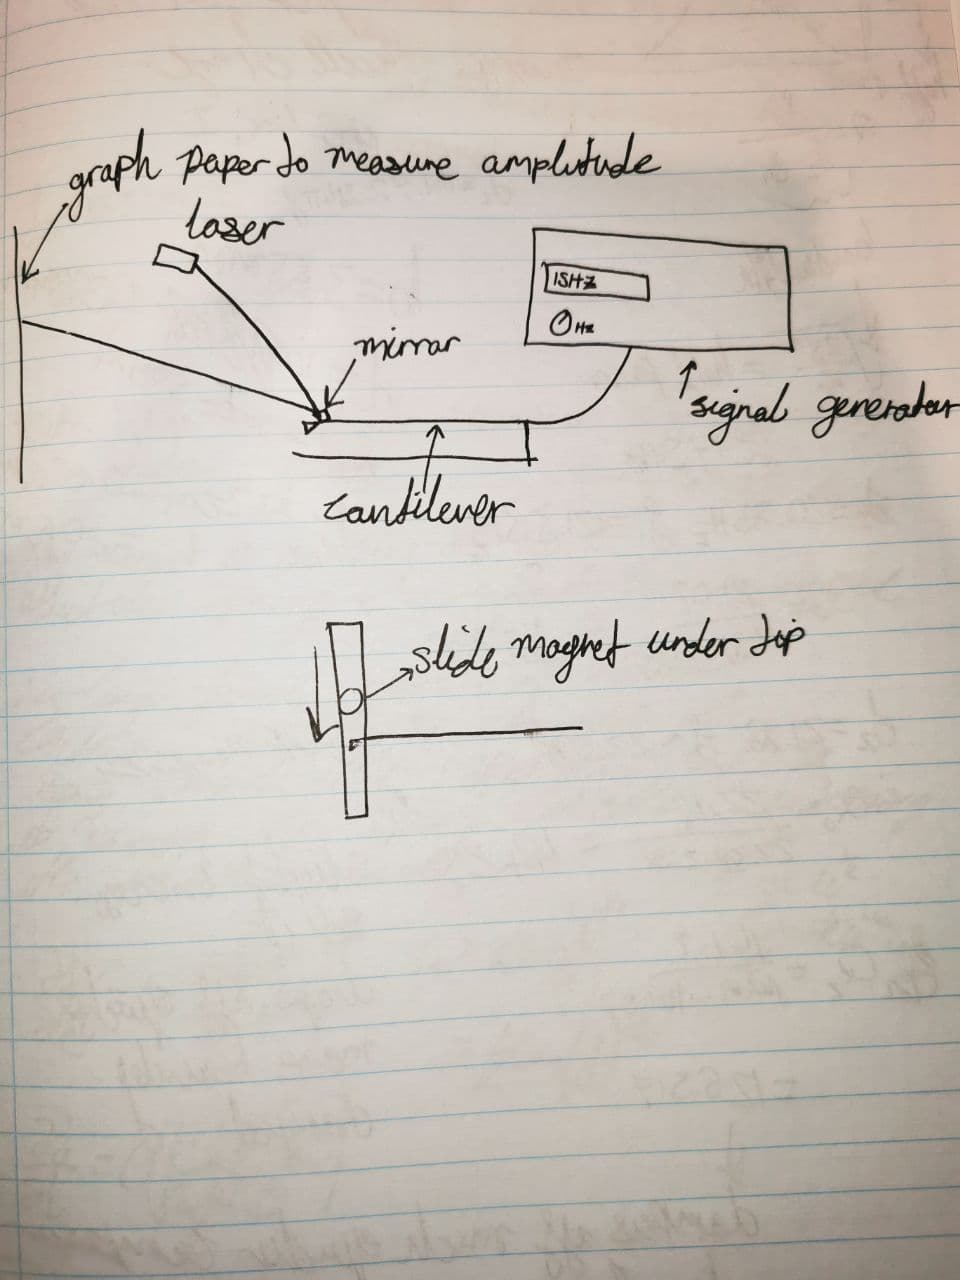
\includegraphics[width=6cm]{fig.jpg}
        \caption{Setup\label{fig}}
    \end{figure}
    \begin{tabular}{l l l}
        Frequency(f) / Hz & Amplitude / cm\\
        18 & 2\\
        20 & 5\\
        20.5 & 10\\
        \vdots & \vdots 
    \end{tabular}

    Plot a resonance frequency curve as shown in Figure: \ref{res}.
    \begin{figure}[h]
        \centering
        \captionsetup{justification=centering}
        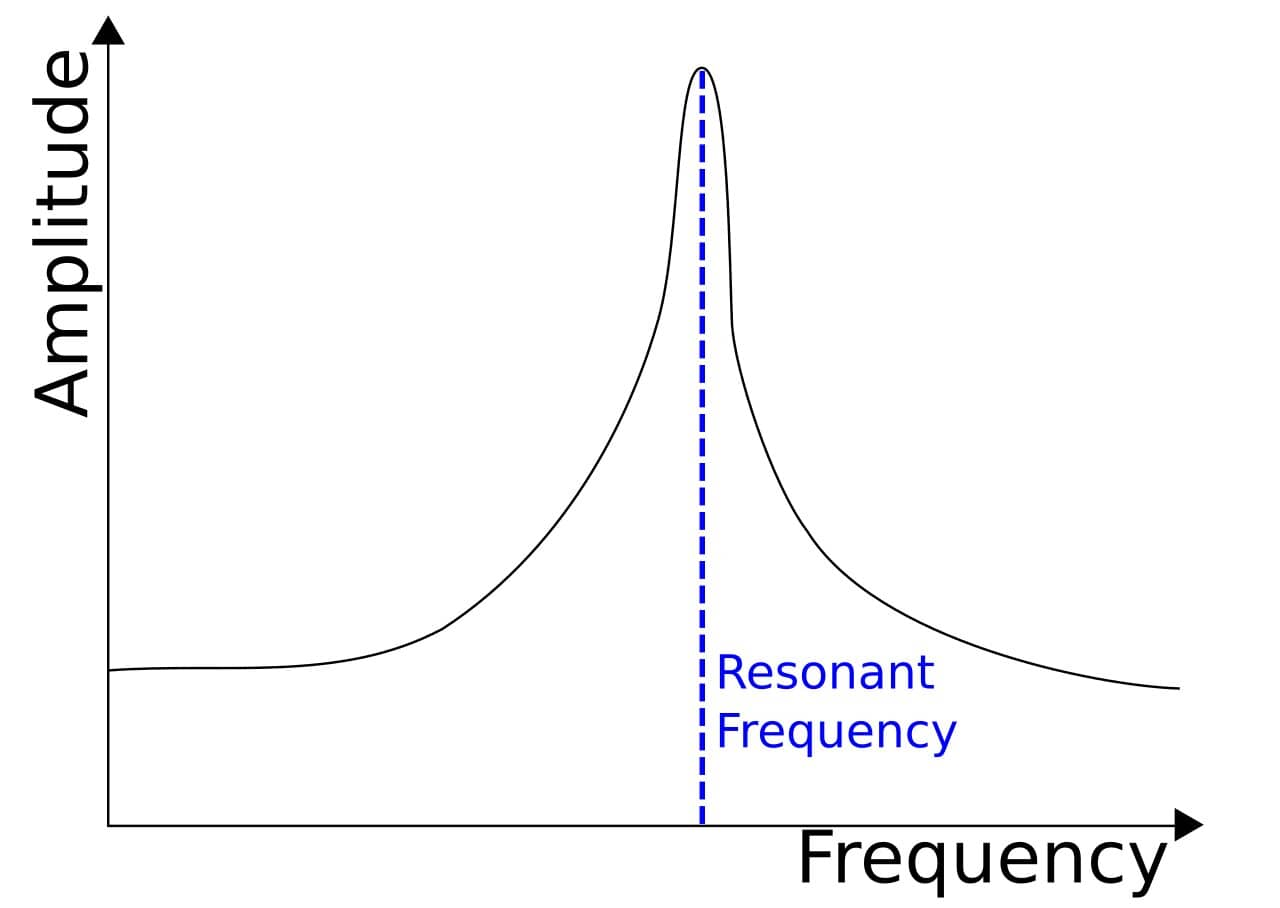
\includegraphics[width=6cm]{res.jpg}
        \caption{Resonance frequency curve \cite{resc} \label{res}}
    \end{figure}
    The Q-value can be calculated by $\frac{f_1}{\text{bandwidth at} 70.7\%}$. This shows how fast an oscilattion 
    will decay, a larger Q value will oscillate for longer. 

    \item Move one of the magnets beneath the tip and again record the fundamental frequency, plot a resonance
    curve and calulate the Q value. How has the fundamental frequency changed?
    \item Find the second harmonic frequency of the cantilever
\end{enumerate}


\newpage
\begin{thebibliography}{9}
    \bibitem{curve}
    nanoscience.com 
    \url{https://www.nanoscience.com/techniques/atomic-force-microscopy/}

    \bibitem{resc}
    wikibooks.com
    \url{https://en.wikibooks.org/wiki/A-level_Physics_(Advancing_Physics)/Resonance/}
\end{thebibliography}

\end{document}


